\documentclass[orientation=landscape]{tikzposter}

\geometry{paperwidth=48in,paperheight=36in}
\makeatletter
\setlength{\TP@visibletextwidth}{\textwidth-2\TP@innermargin}
\setlength{\TP@visibletextheight}{\textheight-2\TP@innermargin}
\makeatother

\usepackage{amsmath,amsthm, amssymb, latexsym}
\usepackage{algpseudocode,algorithm,algorithmicx}

\newcommand*\Let[2]{\State #1 $\gets$ #2}
%%%%%%%%%%%%%%%%%%%%%%%%%%%%%
%%%			Title and Authors			%%%
%%%%%%%%%%%%%%%%%%%%%%%%%%%%%
\title{\parbox{\linewidth}{\centering On Modifications to Laguerre's Method and the Polynomial Eigenvalue Problem}}
\institute{Davidson College \& DiscoverOrg LLC.}
\author{Thomas R. Cameron \& Nikolas I. Steckley}
\usetheme{Rays}
\usebackgroundstyle{Default}
\usetitlestyle{Default}
%%%%%%%%%%%%%%%%%%%%%%%%%%%%%
%%%			Main Document				%%%
%%%%%%%%%%%%%%%%%%%%%%%%%%%%%
\begin{document}
	\maketitle
	%%%	Abstract	%%%
	\block{Abstract}{Laguerre's method has long been recognized for its strong virtues when computing the roots of a polynomial. Over the years, many modifications to Laguerre's method have been suggested in an attempt to improve its convergence rate and to avoid multiple convergence to a simple root. Now, we present a modification to Laguerre's method for the simultaneous convergence of all roots of a polynomial. Multiple numerical experiments verify both the accuracy and efficiency of this algorithm, and we provide comparisons to other root finding methods, such as POLZEROS and AMVW. Furthermore, we are able to apply this method to the polynomial eigenvalue problem, where it is effective for large degree problems, and the Tridiagonal problem.}
	%%%	Column 1	%%%
	\begin{columns}
		\column{0.333}
		%%%	Introduction	%%%
		\block{Introduction}{
			Let $p(\lambda)$ be a polynomial of degree $m$. Denote by $(z_{1},\ldots,z_{m})$ current approximations to the roots, $r_{1},\ldots,r_{m}$ of $p(\lambda)$. Then, for $j\in\{1,\dots,m\}$ define
			\[
			f_{j}(\lambda)=\frac{p(\lambda)}{\prod\limits_{\substack{i=1\\i\neq j}}^{m}(\lambda-z_{i})},
			\]
			and note that $f_{j}(\lambda)$ has the same roots as $p(\lambda)$. Further define
			\begin{equation}
			\begin{split}
			G_{j}(\lambda)&=\frac{f_{j}^{'}(\lambda)}{f_{j}(\lambda)}=\frac{p^{'}(\lambda)}{p(\lambda)}-\sum_{\substack{i=1\\i\neq j}}^{m}\frac{1}{\lambda-z_{i}}, \\
			H_{j}(\lambda)&=-\left(\frac{f_{j}^{'}(\lambda)}{f_{j}(\lambda)}\right)^{'}=-\left(\frac{p^{'}(\lambda)}{p(\lambda)}\right)^{'}-\sum_{\substack{i=1\\i\neq j}}^{m}\frac{1}{(\lambda-z_{i})^{2}}.
			\end{split}
			\end{equation}
			Then the jth root approximation is updated via the expression
			\begin{equation}\label{eq:lag2}
			\hat{z}_{j}=z_{j}-L_{m}(z_{j}),
			\end{equation}
			where the modified Laguerre updated is defined by
			\begin{equation}
			L_{m}(z_{j})=\frac{m}{G_{j}(z_{j})\pm\sqrt{(m-1)(mH_{j}(z_{j})-G_{j}^{2}(z_{j}))}},
			\end{equation}
			and the sign is chosen to maximize the magnitude of the denominator. Note that the modified Laguerre update is effectively the standard Laguerre update applied to $f_{j}(z_{j})$. 
		}
		%%%	Iteration Style and Convergence	%%%
		\block{Modified Laguerre's Method}{
		\begin{algorithmic}[1]
		\For {$k=1 \textrm{ to } itmax$}
		\For {$j=1 \textrm{ to } m$}
		\If{$j$th approximation has not already converged}
			\Let{$z_{j}$}{$z_{j}-L_{m}(z_{j})$}
		\EndIf
		\EndFor
	    \EndFor
		\end{algorithmic}
}	
		\column{0.333}
		\block{Comparisions}{

			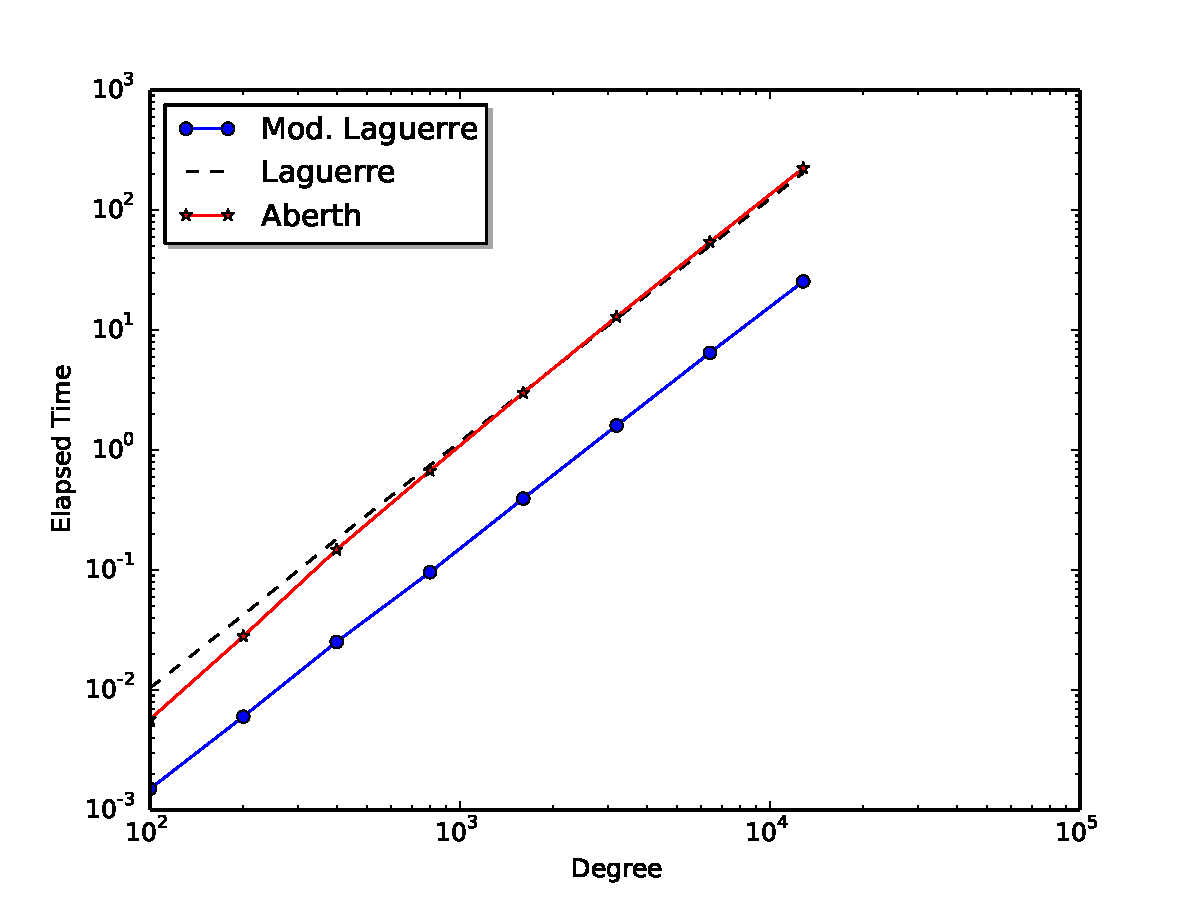
\includegraphics[width=\linewidth]{../develop/tests/diagrams/testMethods}
			\centering *Avgerage of max backward error
			
			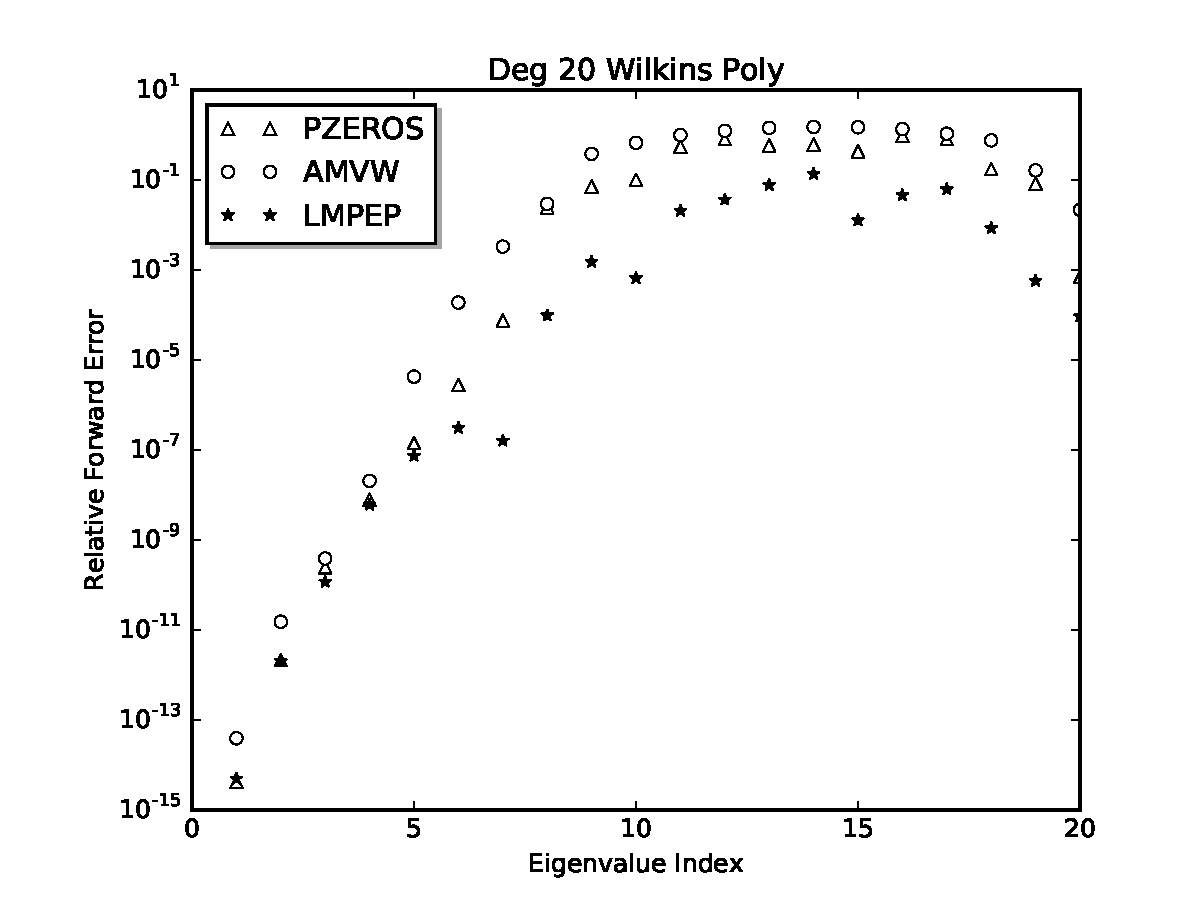
\includegraphics[width=\linewidth]{../develop/research/comparision_test/diagrams/poly_test_Deg_20_Wilkins_Poly.pdf}

		}

		\column{0.333}
		\block{Initial Estimates}{}
		\block{Stopping Criteria}{}
		\block{Order of Convergence}{}
		%\note{Notetext} % See Section 4.3
	\end{columns}
\end{document}